\documentclass[a4paper,8pt,french,fleqn]{report}
%Packages:

%Langages:
\usepackage[french]{babel}
\usepackage{lmodern}
\usepackage[T1]{fontenc}
\usepackage[utf8]{inputenc}

%AMS maths
\usepackage{amsmath, amssymb, amsfonts}

%Mise en page
\usepackage[top=2cm, right=2cm, bottom=2cm, left=2cm]{geometry}
\usepackage{fancyhdr}
\usepackage{enumerate}
\usepackage{color}
%Définition des macros
\usepackage{amsthm}

%Figures
\usepackage{tikz}
\usepackage{graphicx}
\usepackage{wrapfig}

%Symboles mathématiques
\usepackage{latexsym}
\usepackage{bm}

%Listings
\usepackage{listings}
\lstset{language=SQL}

%Titre et auteurs
\title{\textbf{SGBD - Projet Sport }\\\textit{Rapport du travail fourni}}

\author{PHILIPPI Alexande \& MAUPEU Xavier \& PAILLASSA Maxime}

\date{\today}

\begin{document}

\maketitle

\newpage

\tableofcontents

\newpage

\chapter*{Introduction}

Le projet consistait en la réalisation d'une base de données gérant les rencontres entre les clubs de basketball d'une fédération (cf. figure \ref{fig:website}). Il fallait implémenter des requêtes permettant d'obtenir des informations sur les clubs, les équipes et les joueurs. Tel que les meilleurs joueurs, les classements des équipes au sein d'un club et/ou de la fédération. Afin d'intéragir avec la base et la faire évoluer simplement, des scripts d'insertion, de modification et de suppression devaient être implémentés. L'interface entre le client et la base pouvait être implémantée avec n'importe quel langage de n'importe quelle manière tant que cela ne masquait pas les requêtes.

\begin{figure}[h]
  \centering
    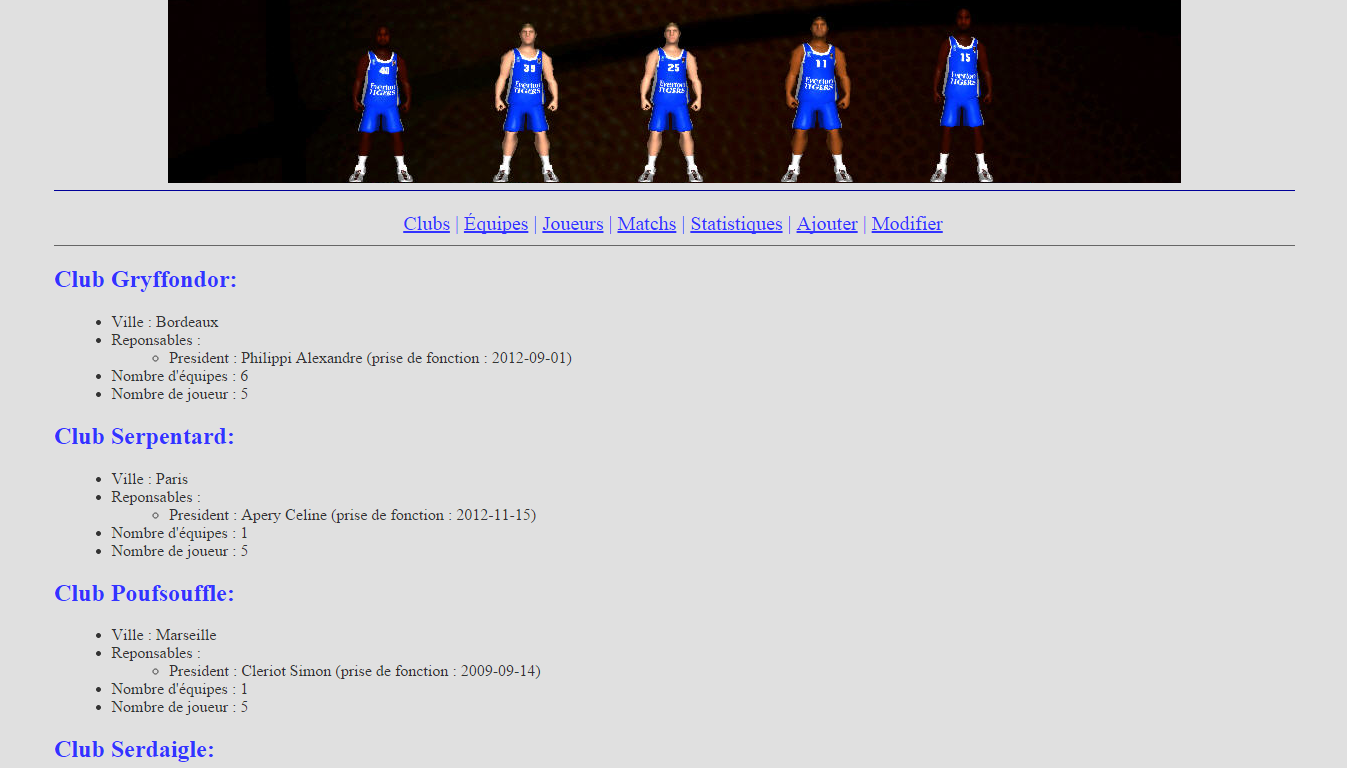
\includegraphics[scale=0.45]{site.png}
    \label{fig:website}
    \caption{Aperçu du site web}
\end{figure}

\chapter{Présentation du modèle}

\section{Description du contexte}

Pour ce projet nous disposons des informations suivantes adaptés de l'énoncé du projet : \\

\begin{itemize}

\item Un club de basket possède un bureau formé d'un président et optionellement d'un trésorier et d'un secrétaire. \\

\item Au sein d'un même club il existe plusieurs catégories et plusieurs équipes de ce club peuvent appartenir à la même catégorie. \\

\item Chaque équipe est composée de plusieurs joueurs lors d'une recontre ou d'un entraînement. Pour un entraînement une équipe a au moins un entraineur. \\

\item Un membre a un nom, un prénom, une date d'entrée et appartient à un unique club. \\

\item Entraineur, joueur et responsable sont des membres. \\

\item Un joueur est également défini par une date de naissance, une adresse et un numéro de licence. \\

\item Un responsable joue un rôle dans le club : Président, trésorier, secrétaire. \\

\item Un entraineur peut entraîner plusieurs équipes du club à des dates différentes. \\

\item Une rencontre est caractérisée par une date, et un numéro. Elle se déroule entre deux équipes. Pour chaque rencontre on associe donc deux équipes, des joueurs affiliés à chaque équipe et un nombre de points marquées et fautes faites affiliés à chaque joueur.

\end{itemize}

\section{Schéma Entité-Association}

\begin{figure}[h]
  \centering
    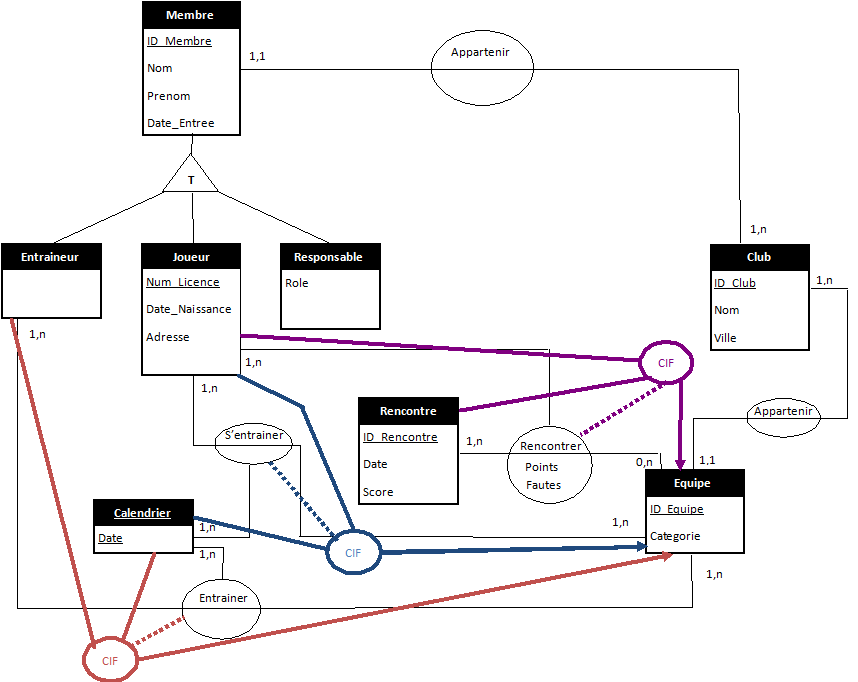
\includegraphics[scale=0.7]{Schema_EA.png}
    \label{fig:schema_ea}
    \caption{Schéma Entité-Association établi par l'équipe}
\end{figure}

D'après la figure \ref{fig:schema_ea}, plusieurs choix ont été fait dans la structuration de la base de données : \\

\begin{itemize}

\item Les joueurs n'appartiennent pas à une équipe mais à un club. Cela offre la possibilité de changer d'équipe un joueur à chaque rencontre. \\

\item Joueur, Responsable et Entraineur héritent de Membre. Par la contrainte de totalité un Membre doit être soit Joueur soit Responsable soit Entraineur, soit deux parmis les trois, soit les trois à la fois.\\

\item La contrainte d'intégrité fonctionnelle appliquée à Joueur et Rencontre permet d'associer un Joueur à une seule équipe lors d'une rencontre. De même pour les entrainements, à une date donnée, un entraineur entraîne une seule équipe et un joueur ne peut s'entraîner qu'avec une équipe. \\

\item Le fait de ne pas lier les points et les fautes uniquement à une rencontre mais également au joueur permet d'aller plus loin dans l'utilisation des données extraites de la base. Cela donne la possibilité d'établir des moyennes de points marqués (ou fautes faites), de voir l'évolution des joueurs au cours des rencontres etc. \\

\item Si plusieurs équipes d'un même club jouent dans la même catégorie, elles sont différenciées par leur ID.

\end{itemize}

\section{Schéma Relationnel}

On peut ensuite passer au schéma relationnel: \\

\begin{itemize}

\item Club(\underline{ID\_Club}, Nom, Ville)  
\item Membre(\underline{ID\_Membre}, \#ID\_Club, Nom, Prenom, Date\_Entree) 
\item Entraineur(\underline{\#ID\_Membre}) 
\item Joueur(\underline{Num\_Licence}, \#ID\_Membre, Date\_Naissance, Adresse) 
\item Responsable(\underline{\#ID\_Membre}) 
\item Rencontre (\underline{ID\_Rencontre}, Date\_Match) 
\item Equipe(\underline{ID\_Equipe}, Categorie, \#ID\_Club) 
\item Rencontrer(\underline{\#ID\_Membre}, \underline{ID\_Rencontre}, \#ID\_Equipe, Points, Fautes) 
\item Sentrainer(\underline{\#ID\_Membre}, \underline{Date\_Entrainement}, \#ID\_Equipe) 
\item Entrainer(\underline{\#ID\_Membre}, \underline{Date\_Entrainement}, \#ID\_Equipe) \\

\end{itemize}

On obtient alors le graphe \ref{fig:depfct} des dépendances fonctionelles.

\begin{figure}[h]
  \centering
    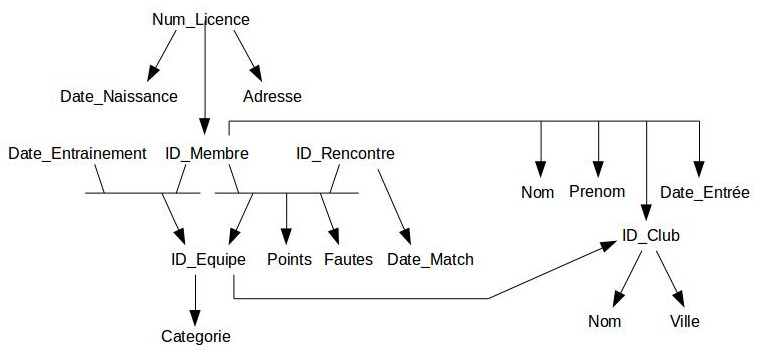
\includegraphics[scale=0.5]{DepFct.jpeg}
    \label{fig:depfct}
    \caption{Graphe de dépendances fonctionnelles}
\end{figure}

On observe ainsi qu'on a la propriété qui nous permet d'affirmer que le schéma est sous 3ème forme normale. En effet, tous les attributs de chaque entité dépendent directement de leur identifiant uniquement. Cela se traduit sur le graphe par le fait que chaque attribut a comme parent(s) direct(s) son identifiant uniquement.

\chapter{Implémentation}

L'interface entre l'utilisateur et la base de données a été faite en PHP. Les sous-parties suivantes présenteront les requêtes implémentées par onglet du site internet.

\section{Clubs}

Cette partie liste les différents clubs de la fédération avec pour renseignement : la ville, les responsables, le nombre d'équipes et le nombre de joueurs. Deux sous-requêtes utilisant la fonction d'agrégation ``COUNT'' sont implémentées dans \ref{club} afin d'obtenir le nombre d'équipes et de joueurs du club. 

\lstset{frame=single, caption={Requete information sur les clubs}, label=club}
\begin{lstlisting}

SELECT c.Nom, c.Ville, c.ID_Club,
       (SELECT count(*) 
        FROM Equipe e
        WHERE c.ID_club = e.ID_Club) AS NombreEquipe,

       (SELECT count(*) 
        FROM Joueur j, Membre m
        WHERE c.ID_Club = m.ID_Club
        AND m.ID_Membre = j.ID_Membre) AS NombreJoueur

FROM Club c;

\end{lstlisting}

\section{Equipes}

Dans l'onglet 'Equipes' il est possible de visualiser le classement des équipes de la fédération par catégorie. La catégorie est séléctionnée via un formulaire PHP et les résultats sont affichés dans un tableau HTML. La fonction d'agrégation ``SUM'' est utilisé afin d'obtenir le nombre de matchs gagnés, ex-aequos et perdus. Une première sous-requête permet d'obtenir le nombre de points marqués par équipe par rencontre. La seconde permet d'avoir le total de points par rencontre. 

\lstset{frame=single, caption={Requête classement des équipes de la fédération par catégorie}, label=equipe}
\begin{lstlisting}

SELECT c.Nom,
       SUM(e.Points > t.Total/2) AS gagne,
       SUM(e.Points = t.Total/2) AS egual,
       SUM(e.Points < t.Total/2) AS perdu
			
FROM ((SELECT ID_Rencontre, e1.*,
       SUM(r1.Points) AS Points
       FROM Equipe e1, Rencontrer r1
       WHERE e1.ID_Equipe = r1.ID_Equipe
       GROUP BY r1.ID_Rencontre, e1.ID_Equipe) e 
                
       INNER JOIN (SELECT ID_Rencontre,
                   SUM(r1.Points) AS Total
                   FROM Rencontrer r1
                   GROUP BY r1.ID_Rencontre) t
                   ON e.ID_Rencontre = t.ID_Rencontre)
 
     INNER JOIN Club c
     ON e.ID_Club = c.ID_Club
			  
WHERE e.Categorie = $_POST['categorie']

GROUP BY e.ID_Equipe
ORDER BY gagne DESC, egual DESC, perdu DESC

\end{lstlisting}

Le classement peut-être restreint aux clubs sans distinction des catégories. La requête est sensiblement la même, si ce n'est que la catégorie n'apparait plus comme un critère de sélection et le nom du club devient le premier critère d'ordonnancement de la table (avant 'gagne', 'egual' et 'perdu'). 


\section{Joueurs}
Dans l'onglet 'Joueurs', les joueurs de la fédération sont classés par clubs avec des informations comme le nom, prénom, numéro de licence... La moyenne des points marqués et des fautes faites, ainsi que leur écart type sont calculés via les fonctions d'agrégation SQL ``AVG'' et ``STD''. La requête \ref{joueur} permet de collecter ces informations dans les tables de la base de données.

\lstset{frame=single, caption={Requête classement des joueurs par club}, label=joueur}
\begin{lstlisting}

SELECT c.Nom AS Nom_Club, 
       m.Date_Entree, m.Nom, m.Prenom, 
       j.Adresse, j.Date_Naissance, j.ID_Membre, j.Num_Licence,
       AVG(rr.Points) AS MoyennePoints,
       STD(rr.Points) AS EcartTypePoints,
       AVG(rr.Fautes) AS MoyenneFautes,
       STD(rr.Fautes) AS EcartTypeFautes

FROM (((Membre m 
        INNER JOIN Joueur j
        ON m.ID_Membre = j.ID_Membre) 
       INNER JOIN Rencontrer rr
       ON rr.ID_Membre = m.ID_Membre)
      INNER JOIN Club c
      ON c.ID_Club = m.ID_Club)
     INNER JOIN Rencontre re
     ON re.ID_Rencontre = rr.ID_Rencontre

WHERE YEAR(re.Date_match) = YEAR(NOW())
GROUP BY c.Nom, j.ID_Membre

\end{lstlisting}

La ligne ``\textit{WHERE YEAR(re.Date\_match) = YEAR(NOW())}'' permet de selectionner seulement les matchs se déroulant pendant la saison courante. Nous sommes partis du principe qu'une saison se déroulait du 1er Janvier d'une année au 31 Décembre de cette même année, pour simplifier les choses.


\section{Graphique}
Grace à l'utilisation de l'extension gd2 de PHP, il est possible de créer des graphiques. Pour chaque mois d'une année et un joueur, sont tracés les points gagnés, les fautes faites et le nombre de matchs gagnés et perdus. La figure \ref{fig:graph} est un exemple de graphique obtenu après application de la requête \ref{graphique}.

\lstset{frame=single, caption={Requête des statistiques pour un joueur}, label=graphique}
\begin{lstlisting}
SELECT Month(Date_Match) AS mois,
       SUM(rr.Points) AS PointsMois,
       SUM(rr.Fautes) AS FautesMois,
       SUM((SELECT SUM(r1.Points)
            FROM Rencontrer r1
            WHERE r1.ID_Rencontre = rr.ID_Rencontre
            AND r1.ID_Equipe = rr.ID_Equipe)
            >
           (SELECT SUM(r1.Points)
            FROM Rencontrer r1
            WHERE r1.ID_Rencontre = rr.ID_Rencontre)/2) AS Gagne,
    
       COUNT(rr.ID_Rencontre) AS NombreMatch

FROM Joueur j, Rencontrer rr, Rencontre re

WHERE j.ID_Membre = $idJoueur
AND   j.ID_Membre = rr.ID_Membre
AND   rr.ID_Rencontre = re.ID_Rencontre
AND   YEAR(Date_Match) = $annee

GROUP BY mois 
ORDER BY mois ASC
\end{lstlisting}

\begin{figure}[h]
  \centering
    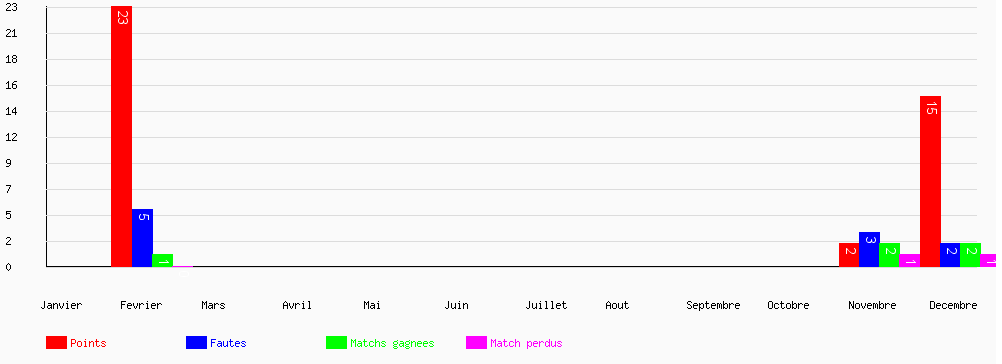
\includegraphics[scale=0.5]{graphe.png}
    \label{fig:graph}
    \caption{Graphique des matchs pour un joueur au cours de la saison 2014}
\end{figure}


\section{Matchs}
Une requête permet de lister les matchs et pour chaque match est affiché le score des deux equipes, la première affichée étant la gagnante.

\lstset{frame=single, caption={Requête des matchs}, label=match}
\begin{lstlisting}

SELECT DISTINCT rr.ID_Equipe, c.Nom, e.Categorie, re.Date_match, re.ID_Rencontre,
                SUM(rr.Points) AS points, 
                SUM(rr.Fautes) AS fautes 
		                      
FROM ((Club c
       INNER JOIN Equipe e
       ON e.ID_Club = c.ID_Club) 
      INNER JOIN Rencontrer rr
      ON e.ID_Equipe = rr.ID_Equipe)
     INNER JOIN Rencontre re
     ON re.ID_Rencontre = rr.ID_Rencontre

GROUP BY e.ID_Equipe, rr.ID_Rencontre
ORDER BY re.Date_match, re.ID_Rencontre, points DESC

\end{lstlisting}

Une autre variante de cette requête permet de sélectionner les matchs par date de rencontre en ajoutant une clause ``WHERE''.


\section{Feuilles de matchs}

Pour chaque match, une feuille de match est créée avec les deux équipes. Les joueurs sont classés par équipe et par nombre de points marqués.

\lstset{frame=single, caption={Requête des matchs}, label=match}
\begin{lstlisting}
SELECT c.Nom as Nom_Club, e.Categorie, m.Nom, m.Prenom, r0.Points, r0.Fautes, 

r0.Points = (SELECT max(Points) 
             FROM Rencontrer r
             WHERE r.ID_Rencontre = r0.ID_Rencontre
             and r.ID_Equipe = r0.ID_Equipe) as MeilleurJoueur,

r0.Fautes = (SELECT max(Fautes) 
             FROM Rencontrer r
	     WHERE r.ID_Rencontre = r0.ID_Rencontre
	     and r.ID_Equipe = r0.ID_Equipe) as PireJoueur 
								
FROM ((((Rencontrer r0 inner join Equipe e
         On e.ID_Equipe = r0.ID_Equipe) 
        inner join Club c            
        On e.ID_Club = c.ID_Club) 
       inner join Membre m
       On r0.ID_Membre = m.ID_Membre) 
      inner join Joueur j
      On m.ID_Membre = j.ID_Membre)

WHERE r0.ID_Rencontre = $id_rencontre
Order by Nom_Club, Points DESC, Fautes ASC
\end{lstlisting}

Lors de l'affichage de cette requête, le meilleur joueur d'une équipe est affiché en vert et celui qui a fait le plus de fautes est affiché en rouge. Ces informations booléennes sont contenues dans les colonnes \textit{MeilleurJoueur}, \textit{PireJoueur}. Elles sont obtenues via un test d'égalité entre le nombre de points (respectivement fautes) d'un joueur et le maximum de points marqués (respectivement fautes faites) déterminés à l'aide de deux sous-requêtes et de la fonction ``MAX''.


\section{Consultation}
A partir d'une date saisie dans un formulaire, l'utilisateur peut rechercher les joueurs inscrits à la date donnée ou alors obtenir le meilleur joueur sur l'ensemble des matchs joués à cette date.\\

\lstset{frame=single, caption={Requête du classement des meilleurs joueurs à une date donnée}, label=consultation}
\begin{lstlisting}
Select m.Nom, m.Prenom,
  sum(r.Points) as Points
				
  From Membre m, Joueur j, Rencontrer r, Rencontre a, Equipe e
  Where m.ID_Membre = j.ID_Membre
    and r.ID_Membre = m.ID_Membre
    and a.ID_Rencontre = r.ID_Rencontre
    and a.Date_Match = $date
    and e.Categorie = $categorie
    and e.ID_Equipe = r.ID_Equipe
   Group by j.ID_Membre
   Order by MoyennePoints DESC
\end{lstlisting}

\section{Ajouter}

Afin de faire évoluer la base de données, des scripts d'ajouts via formulaire PHP ont été implémentés. Il est possible d'ajouter des Membres, des Equipes, des Clubs et des Matchs.

\subsection{Membre}
Pour ajouter un membre, il est nécessaire d'entrer toutes les informations telles que nom, prénom, date de naissance, date d'entrée dans le club, club, activité et poste si responsable. L'adresse n'est pas obligatoire puisque le champs n'est pas à ``NOT NULL'' dans la table Joueur. La validité des dates est vérifiée via une fonction PHP qui teste une chaîne avec une expression régulière. \\

Le club se sélectionne via un menu déroulant pour éviter à l'utilisateur de faire une faute de frappe. Pour ce faire la requête simple ``SELECT Nom FROM Club'' est appliqué à la base de donnée afin de connaître le nom de l'ensemble des clubs. \\

 Pour un membre la sélection d'au moins une activité est obligatoire parmi : Entraineur, Joueur et Responsable, afin de respecter le modèle de l'introduction. Une fois le formulaire rempli et validé, les données sont vérifiées puis insérées dans la base via une requête SQL de type ``INSERT INTO Nom\_Table(...) VALUES (...)''. Dans le cas d'un responsable, afin de vérifier que le poste n'est pas déjà occupé la requête \ref{posteOccupe} est appliquée.

\lstset{frame=single, caption={Requête pour savoir si un poste est occupé}, label=posteOccupe}
\begin{lstlisting}

SELECT Activite

FROM   Responsable r INNER JOIN Membre m
       ON r.ID_Membre = m.ID_Membre

WHERE  m.ID_Club = $id_club
AND    Activite  = $_POST['role']

\end{lstlisting}  

Si jamais le poste est déjà occupé, le nouveau membre est automatiquement supprimé de toutes les tables dans lesquelles il a été créé via une requête SQL de type ``DELETE FROM Table WHERE ID\_Membre = ID\_Nouveau\_Membre''. Ce script ne vérifie pas que la date de naissance du joueur est bien inférieure à sa date d'entrée au club.

\subsection{Club}
Pour ajouter un club, il faut entrer son nom, sa ville et choisir son Président parmi la liste des joueurs et entraîneurs d'autres clubs n'étant pas responsables (Président, Trésorier...). L'établissement de cette liste se fait via la requête \ref{irresponsable}.

\lstset{frame=single, caption={Requête pour connaître la liste des personnes n'étant pas Responsables}, label=irresponsable}
\begin{lstlisting}

SELECT m.ID_Membre, m.Nom, m.Prenom 

FROM Membre m

WHERE NOT EXISTS (SELECT r.ID_Membre 
                  FROM Responsable r 
                  WHERE m.ID_Membre = r.ID_Membre)

\end{lstlisting}  

Comme une personne est déplacée d'un club vers le nouveau il est nécessaire de faire appel à une requête de type ``UPDATE Table SET ID\_Club = ... WHERE ID\_Membre = ...''.

\subsection{Equipe}
L'ajout d'une équipe se fait en choissant un club et une catégorie via deux menus déroulants.

\subsection{Match}
Pour ajouter un match, il faut entrer une date et choisir les deux équipes qui vont se rencontrer. Avant de passer à l'étape suivante, la date et les équipes sont vérifiées. La requête \ref{joueursDispos} permet d'obtenir la liste des joueurs disponibles dans chaque club à cette date. Elle ne vérifie pas que la date de naissance du joueur correspond à la catégorie auquel il est associé. Seul deux équipes de même catégorie peuvent se rencontrer par contre.

\lstset{frame=single, caption={Requête pour connaître la liste des joueurs disponibles}, label=joueursDispos}
\begin{lstlisting}

SELECT DISTINCT m.ID_Membre, m.Nom, m.Prenom, j.Num_Licence, c.Nom AS NomClub 

FROM (Joueur j 
      INNER JOIN Membre m
      ON m.ID_Membre = j.ID_Membre)
     INNER JOIN Club c
     ON m.ID_Club = c.ID_Club

WHERE c.Nom IN ($locaux, $visiteurs)
AND m.ID_Membre NOT IN (SELECT m.ID_Membre

                        FROM (Rencontre re
                              INNER JOIN  Rencontrer rr
                              ON re.ID_Rencontre = rr.ID_Rencontre)
                             INNER JOIN Membre m
                             ON rr.ID_Membre = m.ID_Membre

                        WHERE re.Date_match = $date)

ORDER BY c.Nom

\end{lstlisting}  

Les informations sont ajoutées aux tables Rencontrer et Rencontre avec des fautes et des points attribués de manière aléatoire à chaque joueurs. Le nombre de joueurs participant aux matchs n'est pas vérifié, il est toutefois impossible de ne pas choisir de joueurs pour une équipe. Le nombre minimum de joueurs pouvant jouer est donc un, il n'y a pas de maximum.

\section{Modifier}

La modification de club et d'équipes n'ayant pas beaucoup d'intérêt nous avons décidé de n'implémenter que la modification des membres sans pouvoir toutefois modifier leur rôle en tant que responsable au sein d'un club. Cette décision a été prise pour nous simplifier la tâche par manque de temps. De même la modification de matchs n'est pas prise en compte du fait de la lourdeur de l'implémentation (changement des résultats, validité des résultats, disponibilités des joueurs, ajouts ou retraits de joueurs etc). \\

Dans un premier temps il faut sélectionner le club dont les différents noms sont obtenus via la requête simple ``SELECT Nom, ID\_Club FROM Club'' déjà vu auparavant. Une fois le club sélectionné une autre requête permet d'en obtenir les membres. Enfin, après la sélection du joueur, ses informations s'affichent dans un formulaire pré-rempli grâce à la requête \ref{infosJoueur}.

\lstset{frame=single, caption={Requête pour avoir les informations du joueur}, label=infosJoueur}
\begin{lstlisting}

SELECT r.Activite, m.*, j.Date_Naissance, j.Adresse,

       (SELECT COUNT(*) 
        FROM Entraineur e1
        WHERE e1.ID_Membre = $id_membre) AS entraine,

       (SELECT COUNT(*)
        FROM Joueur j1
        WHERE j1.ID_Membre = $id_membre) AS joue,

       (SELECT COUNT(*)
        FROM Responsable r1
        WHERE r1.ID_Membre = $id_membre) AS gere


FROM (Membre m 
      INNER JOIN Joueur j
      ON j.ID_Membre = m.ID_Membre)
     LEFT OUTER JOIN Responsable r
     ON r.ID_Membre = $id_membre
     
WHERE m.ID_Membre = $id_membre

\end{lstlisting}  

\chapter{Utilisation}

Le projet a été réalisé comme un site web fonctionnant sous PHP avec les extensions PDO\_MYSQL et GD2. La base de données a été implémentée dans MySQL. Nos tests ont été faits avec un serveur Apache 2.4.9, PHP 5.5.12 et MySQL 5.6.17. \\

Après vous être identifié dans MySQL, il faut créer la base de données ``basketball'' et charger les tables contenues dans le fichier ``base.sql''. Il faut ensuite injecter les données contenues dans ``donnees.sql''. De base le login pour la base de données est 'root' et il n'y a aucun mot de passe de défini. Ces informations peuvent être modifiées dans ``Database.php''. \\

La page de garde du site est ``index.php''.

\chapter*{Conclusion}

Ce projet nous a permis de mettre en pratique les connaissances apprises sur les bases de données. Nous avons pu nous rendre compte que prévoir un bon modèle n'est pas facile et que chaque choix d'implémentation a des avantages et des inconvénients. L'insertion de requetes SQL se fait sans réels problèmes en PHP mais les scripts d'ajouts et de modification deviennent vite assez lourds lorsque l'on prend en compte la vérification des données entrées pour s'assurer de leur bonne insertion dans la base de données. Une première évolution serait la mise en place d'une vue afin de connaître l'âge des joueurs pour pouvoir gérer correctement les catégories lors des matchs. Bien qu'implémentée en tant que table dans la base de données, Sentrainer n'a pas été utilisé dans ce projet, nous pourrions également envisager de développer cette partie.

\end{document}
